% Example thesis demonstrating cslu-thesis.cls usage
%
% Document options:
%
% copyright - include a copyright page
% listoftables - include a list of tables
% listoffigures - include a list of figures
% twoside - format for two-sided printing and binding
% masters - generate a Master's thesis instead of a Ph.D. thesis
%
% All other options are passed to the underlying report class, e.g., 10pt
\documentclass[copyright,masters]{cslu-thesis}

\usepackage{lipsum} % for placeholder content text only
\usepackage{tabularx}
\usepackage{graphicx}
\usepackage{amssymb,amsmath,bm}
\usepackage{textcomp}
\usepackage{tkz-graph}
\usepackage{enumitem}
\usepackage{listings}
\usepackage{booktabs}
\usepackage{array}
\usepackage{multirow}


\GraphInit[vstyle = Shade]
\tikzset{
  LabelStyle/.style = { rectangle, rounded corners, draw,
                        minimum width = 2em, fill = yellow!50,
                        text = red, font = \bfseries },
  VertexStyle/.append style = { inner sep=5pt,
                                font = \Large\bfseries},
  EdgeStyle/.append style = {->, bend left} }

\def\vec#1{\ensuremath{\bm{{#1}}}}
\def\mat#1{\vec{#1}}


\lstset{language=Java,
  showstringspaces=false,
  columns=flexible,
  basicstyle={\small\ttfamily},
  numbers=none,
  numberstyle=\tiny\color{gray},
  keywordstyle=\color{blue},
  commentstyle=\color{dkgreen},
  stringstyle=\color{mauve},
  breaklines=false,
  breakatwhitespace=false,
  tabsize=3
}


\newcommand\MyBox[2]{
  \fbox{\lower0.75cm
    \vbox to 1.7cm{\vfil
      \hbox to 1.7cm{\hfil\parbox{1.4cm}{#1\\#2}\hfil}
      \vfil}%
  }%
}


\begin{document}


% Required info for title page and elsewhere
\title{Using Past Speaker Behavior to Better Predict Turn Transitions}
\author{Tomer M.\ Sagie Meshorer}
\previousdegrees{B.\,A. Computer Science, Tel Aviv University, 1997}
\discipline{Computer Science \& Engineering}
% Advisor, readers are in {Name}{Title} format
% Fourth reader is optional; all others are required
\principaladvisor{Prof. Peter A. Heeman}{Research Associate Professor}
\firstreader{Steven Bedrick}{Assistant Professor}
\secondreader{Stephen Wu}{Assistant Professor}
%\thirdreader{NA}{NA}
% Date degree will be conferred
\degreedate{June}{2017}
% Override the default department if needed
% Default is "Center for Spoken Language Understanding"
%\renewcommand{\department}{Department of Biomedical Engineering}


% Front matter
% Title, copyright, signature pages
% See document options above
\frontmatter


% Additional preface sections (optional)
\prefacesection{Dedication}
I would like to dedicate this work to my father, Israel Sagie $(1945-2016)$, who passed away during the preparation of this work.
His wisdom and support will always guide me.
\prefacesection{Acknowledgements}
I would like to express my deep appreciation to Prof. Peter Heeman for his guidance during this research. Without his valuable assistance,
I could not have completed this work.

I would also like to express my appreciation to the members of the committee, Prof. Steven Bedrick and Prof. Stephen Wu, for reviewing
the work and providing invaluable feedback.

I am also indebted to the staff and students of the Center of Spoken Language Understanding, and especially to the gradate program coordinator, Ms. Patricia Dickerson,
for her valuable assistance during the course of my studies.
This work was partially funded by the National Science Foundation under grant IIS-1321146.


% Table of contents, lists of tables/figures
% See document options above
\tableofcontents


% Abstract
\abstract
 Conversations are at the core of everyday social interactions. The interactions between conversants are preformed within the realm of a sophisticated and self-managed turn taking system. In human conversations, the turn taking system  supports minimal speaker overlap during turn transitions and minimum gaps between turns. Spoken dialogue systems are a new form of conversational user interface that permits users to use their voice to interact with the computer. As such, the turn taking capabilities of SDS should evolve from a simple timeout to a more human-like model. Recent advances in turn taking systems for SDS use different local features of the last few utterances to predict turn transition.

This thesis explores using a summary of past speaker behavior to better predict turn transitions. We believe that the summary features represent an evolving model of the other conversant. For example, speakers who typically use long turns will be likely to use long turns in the future. In addition, speakers with more control of the conversation floor will be less likely to yield the turn. As the conversational image of the speaker evolves as the conversation progresses, other speakers might adjust their turn taking behavior in response.

We computed two types of summary features that represent the current speaker's past turn-taking behavior: \textit{relative turn length} and \textit{relative floor control}. Relative turn length measures the current turn length so far (in seconds and words) relative to the speaker's average turn length. Relative floor control measures the speaker's control of the conversation floor (in seconds and words) relative to the total conversation length. The features are recomputed for each dialog act based on past turns of the speaker within the current conversation. Using the switchboard corpus, we trained two models to predict turn transitions: one with just local features (e.g., current speech act, previous speech act) and one that added the summary features. Our results shows that using the summary features improves turn transition prediction.


 % Main body
\body


\part{Introduction} % parts are optional, just chapters are OK too

\chapter{Introduction}
\label{chap:intorduction}
Conversations are a frequent form of everyday social interaction and are characterized by rapid exchange of messages between the conversants.
The turn exchange system in human conversation is universal in nature and crosses culture, age and language \cite{levinson2016turn}. According to the
seminal work by Sack et al. \cite{sacks1974simplest}, a single speaker controls the conversation floor the majority of time in a conversation, conversants takes turns, and the gap and overlap between turns is kept to a minimum. These attributes apply regardless of turn length (from a single word to a full sentence) and conversation length.

In this work we are interested in the point of possible transition between speakers. To keep the gaps between turns minimal while supporting speaker change, the listener
must predict a possible turn transition before the end of the speaker's utterance. Two dominating approaches tried to explain the mechanisms by which
the conversation floor is allocated. Duncan \cite{duncan1972some} suggested that the speaker signals the listener about an upcoming turn transition by using a combination of one or more signals.
Another approach, suggested by Sacks et al.~\cite{sacks1974simplest}, defines the turn allocation process in terms of a set of local rules that are operated at possible turn transition points.
Both approaches (signaling and turn allocation rules) are based on phenomena that occur in the last few utterances (for example, the syntactic construct of the turn or the use of an adjacency pair). This work investigates whether using features that were computed over all past turns can help to improve the predictability of turn transition.

Spoken dialogue systems (SDS) are computer systems that support a conversional speech-based user interface. Users engage in a conversation with the computer to
perform a task (for example, information seeking) by using their natural apparatus, the voice. Hence, to be effective and user friendly, an SDS should also adhere to the system of turn exchange.

Early SDS systems did not contain a turn management component and instead used a fixed timeout to detect the end of a user turn. Using a simple timeout led to barge-in situations, in which the system prematurely started to speak during the user's turn. Decreasing the barge-ins by increasing the timeout caused large gaps between turns, where the user waited for the system to speak.
To improve this situation, newer SDS systems are incorporating recent findings in human-human conversation in their prediction models. For example, features from the latest utterance are used to predict turn transition. Prediction in human-human conversation is based on syntactic \cite{sacks1974simplest,de2006projecting}, prosodic  \cite{ford1996interactional,stolcke2002speaker,ferrer2003prosody}, pragmatic cues  \cite{ford2001intersection}.
% introducing current research

While local features of the latest utterance form an important input for prediction, this thesis postulates that speakers might also use summary features computed over many turns. The summary features form a conversational image of the speaker and contain features that represent the speaker's average behavior over many turns. For example, average turn length measures the length in both time and words of each converstants turn up to this turn. Hence, if the length of the current speaker's turn is more than its average turn length, it is more likely that a turn ending will occur.







\section{Thesis Statement}
This work investigates whether summary features based on past speaker behavior in a conversation can help improve turn transition prediction. 
Using the switchboard corpus, we computed for every dialog act in the conversation two summary features: \textit{relative turn length} of the current turn, and the \textit{relative floor control}.
In addition, after each dialog act in the conversation, we marked whether a turn transition occurred. Our hypothesis is that we can make better
turn transitions by using the summary features, compared to using only local features.  
  
\section{Approach}
To test the effectiveness of the summary features, we used the NXT version of the Switchboard corpus \cite{calhoun2010nxt,Godfrey-etal92:icassp} to train random forest models \cite{scikit-learn}. First we performed data preprocessing in order to merge turn, dialog act and single word information into a single data set. Next, we trained baseline models using local features: current and previous dialog acts. We also trained a model on the summary features as well as a model that includes both the local and the summary features. To measure the predictive power of the different models we use standard model metrics: F1, precision, recall and area under the curve (AUC)


\section{Contribution}
Our results show that the summary features improve prediction performance in both area under the curve (AUC), $69.4\%$ vs $66\%$, and F1, $69.3\%$ vs $57.8\%$. In addition, the model that was trained on all of the features performs better than the local features model in both AUC, $83.7\%$ vs $81.1\%$, and F1, $77.5\%$ vs $74.8\%$. The results show that using summary features helps predict turn transitions.


\section{Dissertation Structure}
Chapter 1 contains the introduction, the definition of the summary features and the thesis statement. Chapter 2 presents the related work in both human-human and human-computer conversations. Chapter 3 describes the theoretical model the underline the summary features. Chapter 5 describe the data sources, data preparation and initial data analysis. Chapter 5 describes the study which compute the long term features over all the turns in each conversations. The chapter describes the experiment and includes the description of the corpus, the data preparation pipeline, and the result, which compares the baseline models as well as the model that includes the summary features. Finally, in chapter 6 we present the conclusion and future work.


This work is based on Meshorer and Heeman \cite{Meshorer2016UsingPS} which was submitted and presented in interspeech 2016.

\chapter{Related Work}
This chapter presents work related to turn transition prediction in both human-human conversations and human-computer conversations. Studying human-human turn allocation mechanism might
%
inform us on the inner workings of the system that people use
%
during conversations when regulating turn allocation. This in turn
%
will help guide us in
%
how to implement such mechanisms in spoken dialogue systems.


\section{Human-Human Conversations}
Duncan \cite{duncan1972some} argued that speakers signal when they want the listener to take the turn and presented six signals used by the speaker to accomplish this: intonation, drawl on the final syllable, body motion, sociocentric sequence, drop in pitch or loudness, and syntax. Kendon \cite{kendon1967some} added gaze as a signal to turn transition. Our summary features complement the set of signals as suggested by \cite{duncan1972some}.


Turn allocation was introduced in the seminal work by Sacks, Schegloff, and Jefferson \cite{sacks1974simplest}, who observed that conversations are ``one speaker at a time'' and gaps between turns as well as speaker overlaps are kept to a minimum. To satisfy these constraints, Sacks et al.~suggested an ordered set of rules for turn allocation:
%
(a) current speaker selects the next conversant; (b) if the current speaker did not select, any of the listeners can self select; or (c) if neither of the previous two cases apply, the current speaker continues.
%
For the first rule, Sacks et al.~suggested that the current speaker uses adjacency pairs as the main apparatus for selecting the next speaker. Hence, we recognized the importance of dialog acts in turn allocation and chose them as the atomic turn components. In addition, our work might impact the second rule, in which the conversant self selects. While Sacks et al.~suggested that the first starter is the next speaker, we suggest that a conversant might use the conversational image of the speaker and of themselves when self selecting. For example, a controlling speaker (with a high relative floor control score) has a better chance to gain control of the conversation floor when self selecting.  The work on turn bidding is also related \cite{SelfridgeHeeman10:acl}, which suggested that each conversant measures the importance of their utterance when negotiating the right to the conversation floor.

In addition to the turn allocation system, Sacks et al.~also suggested that turn construction units (TCU) should support projection of turn ends by the participants. The projectability attribute was later extended to other features of the speaker's utterance: (syntactic \cite{sacks1974simplest}, prosodic \cite{ford1996interactional} and pragmatic \cite{ford1996interactional,ford2001intersection}). Our work augments the local utterance features with summary features that can be used to improve projectablity.

Entrainment was presented in \cite{wilson2005oscillator}, which suggested entrainment of endogenous oscillators in the brains of the speaker and the listener on the basis of the speaker syllabus production. In their study, the speaker and the listener are counter phased such that speech overlaps and gaps are minimized. Although our work does not imply cyclic synchronization between speaker and listener, we do suggest that each conversant creates a conversation image of the other conversant and uses it during turn transition.

The importance of using dialog acts was emphasized by a very recent study of Garrod and Pickering \cite{garrod2015use}. The study suggested that turn production is a multi-stage process in which the listener performs simultaneous comprehension of the existing turn as well as production of the new turn content. They suggested that the first step in the process is dialog act recognition, which is done as soon as possible and acts as the basis for the listener's turn articulation and production. In our study we use dialog act as the main turn component.


\section{Human-Computer Conversations}

As recent advances in machine learning reduce speech recognition error rates, the problem of turn taking in SDS rises in importance \cite{hinton2012deep}. Traditional SDS systems use a simple silence timeout approach to trigger turn transitions. This creates three issues \cite{arsikere2015enhanced} first, the model might not be robust enough
in a noisy environment (for example when driving); second, if the timeout is too short, the system might
detect intra-turn pauses (for example, the user pausing to think) as a turn transition and will cut into the user's turn;
and third, if the timeout is too long the system will wait too long to take the turn, resulting in large gaps between turns.

Recent studies tried to improve over the simple threshold model by using machine learning to train models based on features derived from the latest utterance. As different studies use a variety of features, we will outline those that used counting features that are close to the summary features.

Arsikere et al.~\cite{atterer2008towards} focused on utterance segmentation in the context of an incremental dialog system.
Using the switchboard corpus, they used a decision tree algorithm to decide if a word is the final utterance by using various features and in particular the number of words in the turn so far. The usage of count features improves precision by 10\% but has very low recall (7\%), which might have occurred, according to the author, from turns with only one word.

Gravano and Hirschberg \cite{gravano2011turn} used the Columbia games corpus to study the effectiveness of
different turn transition cues. The authors define inter-pausal units (IPU) as a maximum sequence of words surrounded
by silence of more than 50 ms. A turn is the longest sequence of IPUs by the same speaker.
One of the features studied is IPU duration in ms as well as number of words. As in our findings,
the authors found that long IPUs are a good indication of upcoming turn changes (long IPUs might correlate with a speaker passing
its average turn length). Moreover, as we show in Section 5, the authors found that combining multiple cues leads to better accuracy.

Raux and Eskenazi \cite{raux2012optimizing} performed a comprehensive study of features that inform turn changes. The study
found that timing features, such as turn duration and number of pauses, have relatively strong predictive power. While Raux and Eskenazi use features of the current turn, in our study we use the timing features for the turns that have occurred so far in the current conversation.

Ina more recent study, Nishitha and Rodney \cite{SSS1510313} used a model based on N grams of dialog acts to predict turn transitions.
They trained a decision tree model using the switchboard data and tested bigram, trigram and 4 grams models of
dialog acts with and without speaker id. They achieved an F1 measure of $0.67$ for the trigram model.
In this paper, we based our baseline models on bigrams and trigrams of dialog acts.  We also mapped the switchboard dialog acts from 148 dialog acts down to 9 to reduce data dimensionality. The prediction performance of our baseline model is comparable to their results.


\chapter{Theoretical model}
This chapter aims to provide a more formal description of our turn taking model. First we present a formal definition of a conversation, turn changes and local features. Next we present the formulas to compute the summary features: relative turn length and relative floor control.

\section{Local Features}

     We define a conversation as a sequence of dialogue acts $d_1 \dots d_N$, where $d_i$ is uttered by speaker $s_i$.  We write this as the following sequence:
%
     \begin{equation}
       \ldots  s_{i-2}, d_{i-2}, s_{i-1} , d_{i-1}, s_i, d_i  \ldots
     \end{equation}
     We denote whether there was a turn transition with $y_i$. A turn transition occurs when the speaker $s_i$ is different from speaker $s_{i-1}$. Hence, (1) can be also be viewed as a sequence of dialog acts $d_i$ followed by turn transitions $y_i$:
%
     \begin{equation}
       \ldots    d_{i-2}, y_{i-1}, d_{i-1}, y_{i} , d_i, y_{i+1} \ldots
     \end{equation}
      In our first baseline model, we try to predict the turn transition value $y_{i+1}$ based only on the latest dialog act $d_i$. In our second baseline model, we try to predict turn transition $y_{i+1}$ based on the latest two dialog acts: $d_{i-1}$ and $d_i$.


\section{Summary Features}\label{sfeatures}

     As discussed in the introduction, we introduce two types of summary features in this paper: relative turn length ($rt_i$) and relative floor control ($rc_i$).  These features are used in predicting whether there is a change in speaker $y_{i+1}$ after dialogue act $d_i$.

     To compute the summary features at dialogue act $d_i$, we introduce some notation. Let $S_i$ to be the set of complete turns of speaker $s_i$ that are prior to the turn that $d_i$ is in.  Let $t_i$ represent the turn so far that $d_i$ is in, up to $d_i$ but no subsequent dialogue acts.  Let length(t) be the length of a turn or a partial turn in seconds (or words). To compute the \textit{relative turn length} of turn $t_i$ we first compute the average length of all the turns in $S_i$
%
    \begin{equation}
     avg\_t_i = \frac{\sum_{t \in S_i} length(t)}{|S_i|}
     \end{equation}
     The \textit{relative turn length} summary feature of $t_i$, denoted as $rt_i$, measures the percent of the length of the turn $t_i$ so far, relative to the average turn length up to $t_i$ of the current speaker $s_i$ (but not including $t_i$).
%
     \begin{equation}
            rt_i =  \frac{length(t_i)} {avg\_t_i}
     \end{equation}
     Note that we calculate two versions of $rt_i$: in seconds and in words.  The purpose of $rt_i$ is to let the listener, in predicting turn changes, take into account whether the current speaker is exceeding his or her average turn length.

     The \textit{relative floor control}, denoted as $rc_i$, measures the percent of time in which the current speaker controlled the conversation floor up to $d_i$. We use $S_i$ as defined above:
     the set of complete turns of speaker $s_i$ that are prior to the turn that $d_i$ is in.
     %
     We similarly define $L_i$ to be the turns of the other conversant (the listener of $d_i$) that are prior to $d_i$.
     %
     We first compute the conversation length up to $d_i$ denoted as $c_i$, which excludes inter-utterance pauses but includes intra-utterance pauses.
     \begin{equation}
         c_i = \sum_{t \in S_i \cup L_i} length(t)
     \end{equation}
     To compute relative floor control at $d_i$, we divide the floor time of the speaker $s_i$ up to turn $t_i$ by $c_i$:

     \begin{equation}
        rc_i = \frac{\sum_{t \in S_i} length(t)} {c_i}
     \end{equation}
     Note that we also calculate $rc_i$ in seconds and in words. Participants can use the relative floor control as a means to determine if one speaker is controlling the conversation; a controlling speaker will probably be less inclined to give up the floor.

     We use these two summary features in the \textit{summary model} and \textit{full model}, as described in Chapter 5.



\chapter{Data}
To evaluate the importance of the summary features in predicting turn transitions we used the 2010 version of the switchboard corpus \cite{calhoun2010nxt} which is based on the original release \cite{225858}.

The switchboard corpus is the first large collection of phone conversations and was collected in 1990-1991. The initial goal of the corpus is to facilitate speech research by providing pre recorded audio files of day to day conversations. The original corpus was composed of 2483 phone calls involving 520 speakers. Each call ranged from 1.5 minutes to 10 minutes, with an average length of 6 minutes. Conversations involved a randomly chosen topic between two randomly selected speakers. The corpus was later improved and was released as part of the Penn Treebank 3 corpus, which included 650 annotated conversations. The current release used for this research includes 642 conversations and just over 830000 words.

The current corpus contains multiple annotations for each conversation. We used the turns annotation to assign turns to speakers and mark the turn start and end points. We used the dialog act annotation to assign dialog acts to turns such that each turn interval contain all the dialog acts that occured between turn start and turn end. Next, we use the token annotation to assigned words to dialog acts and to compute the overall number of words within each dialog act.

\section{Data Preparation}
    Figure \ref{pipeline} shows our data pipeline. Data is imported from the NXT switchboard corpus \cite{calhoun2010nxt} into a graph database \cite{Webber:2012:PIN:2384716.2384777}.
   Figure \ref{datastructure} shows the data structure as it is represented inside the graph database. For each conversation, the conversation entities (words, dialog acts and turns) are represented as edges between time points, which are represented as vertices. The structure leads to a direct computation of the summary features using the graph query language.
\begin{figure}[ht!]
 \centering
 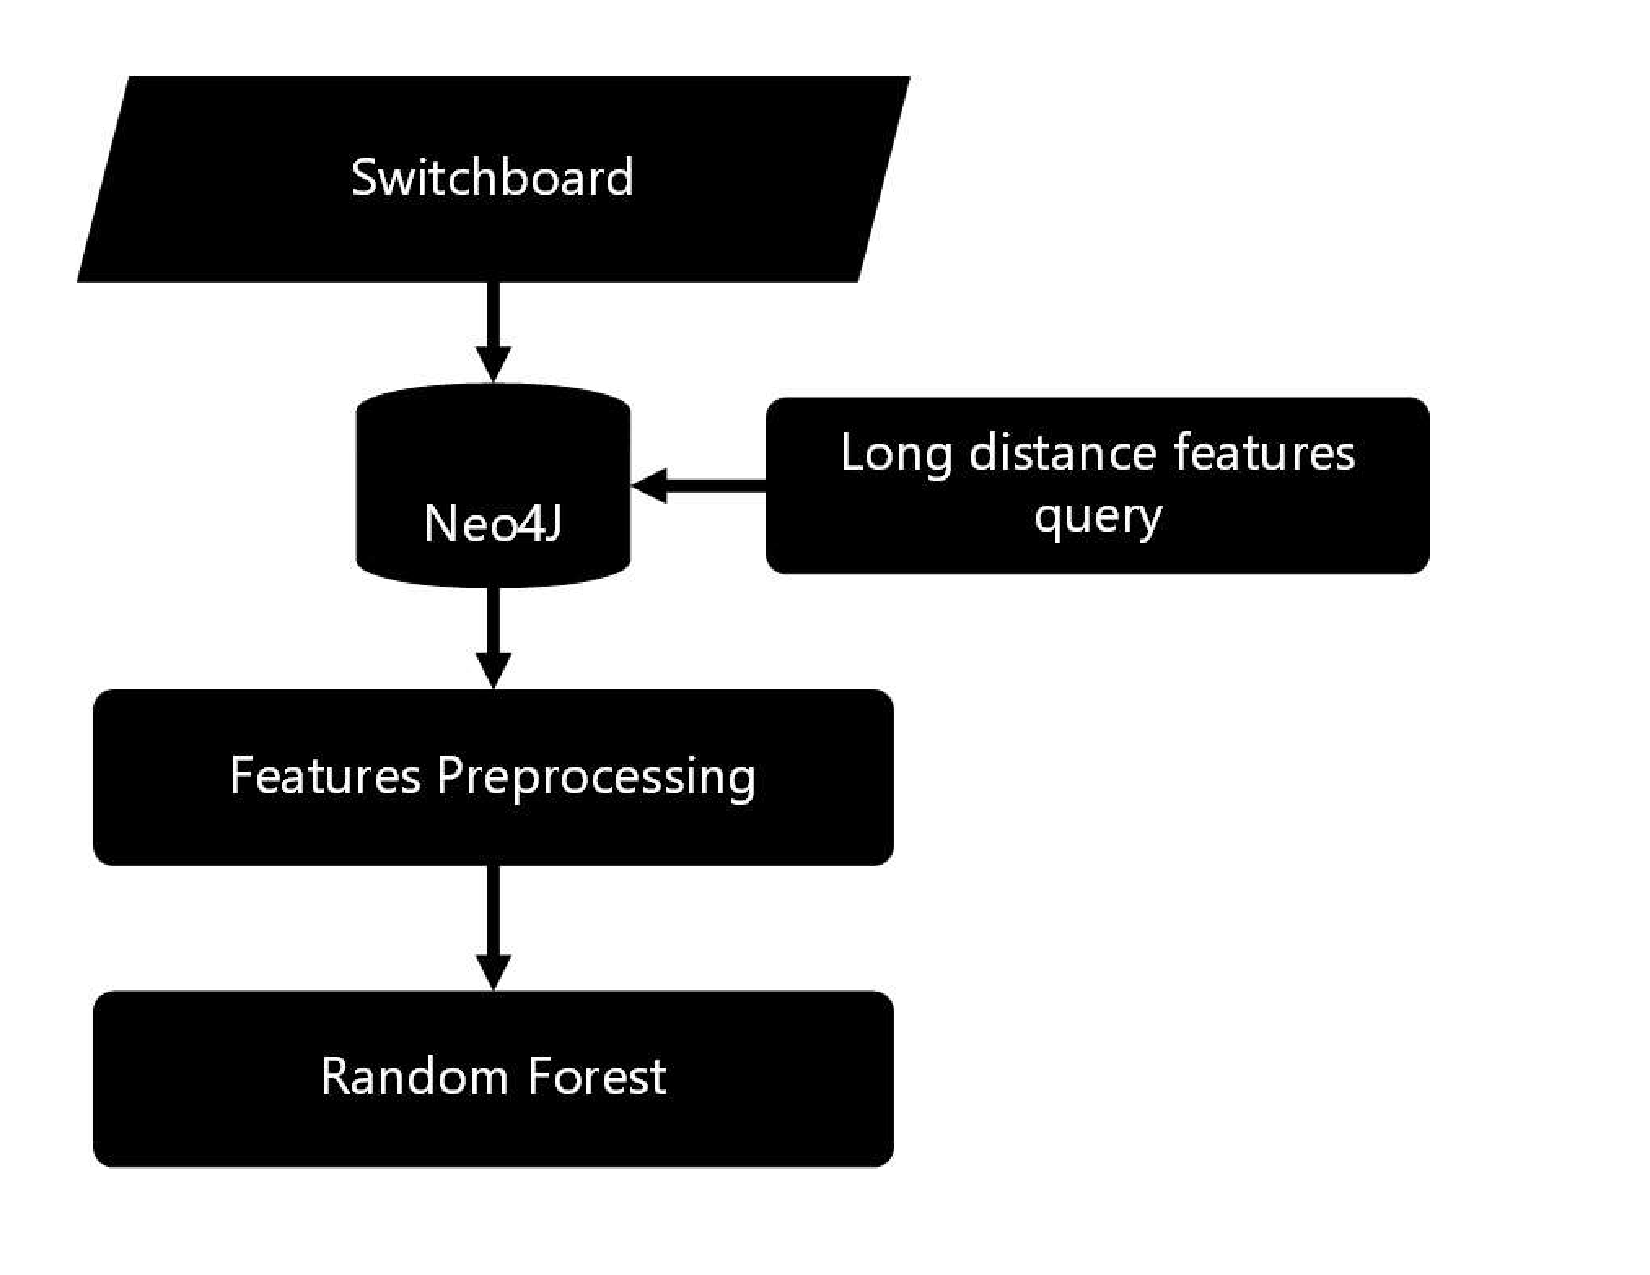
\includegraphics[width=10cm,keepaspectratio]{pipeline1.pdf}
 \caption{Experiment data pipeline
 \label{pipeline}}
 \end{figure}



\begin{figure}[ht!]
\centering
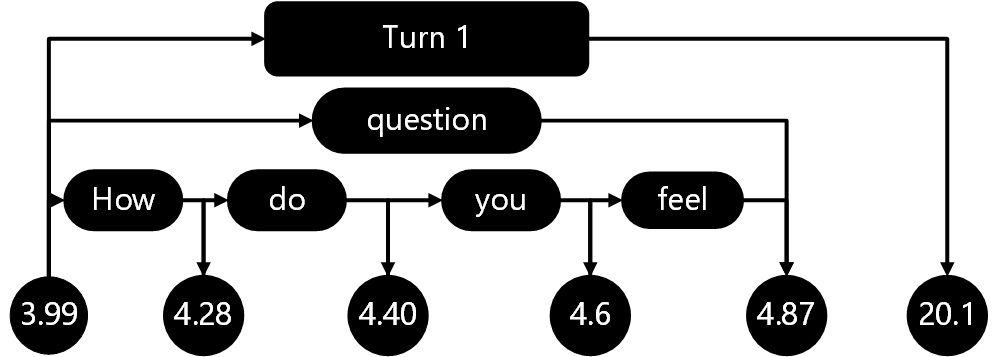
\includegraphics[width=10cm,keepaspectratio]{graph5.jpg}
\caption{Conversation graph data model \label{datastructure}}
\end{figure}

   After computing the summary features, we perform the following data transformation:
    \begin{itemize}[leftmargin=1em]
    \item We exclude 11 dialogue acts that were coded in Switchboard as ``other.''
    \item We filtered out all the dialogs that had data integrity issues,  for example
          dialog acts that referred to non existent terminals. This decrease the number
          of conversations from 624 to 310 conversations consisting of 60595 dialog acts.
    \item To reduce data sparsity, we grouped switchboard dialog acts into dialog act classes. This reduced the number of dialog acts from 148 to 9 dialog act classes. See Table 1 for examples of the mapping.
    \item We added a binary $y_{i+1}$ feature to each dialog act. As explained in Section 3, the variable is 1 if there is a turn change from dialogue act $d_i$ to $d_{i+1}$.

    \end{itemize}
    \begin{table}
     \begin{center}
    \begin{tabular}{ |p{2cm}||p{3cm} | }
    \hline
Switchboard dialog acts &  Dialog act classes  \\
    \hline
sd,h,bf      & statement   \\
sv,ad,sv@    & statement - opinion  \\
aa,aa\^r     & agree accept \\
\%.\%-,\%@   & abandon      \\
b,bh         & backchannel  \\
qy,qo,qh     & question     \\
no,ny,ng,arp & answer       \\
+            & +            \\
o@,+@        & NA           \\
  \hline
\end{tabular}
\end{center}\vspace{-0.5em}
\caption{Mapping from dialog act to dialog act class}
\label{tab:mapping}
\end{table}

\section{Data Exploration}
Before performing the actual learning and prediction tasks, this chapter explores the data
in order to understand the statistics of the different features.

\subsection{Features}

After pre processing the data the data set to be explorted is describe in the following table:

\begin{table}[ht!]
\begin{center}
\begin{tabular}{llllrr}
\toprule
Field &  Description & Type &\\
\midrule
     Previous Dialog Act & dialog act before the current one  & categorical\\
     Dialog Act & current dialog act & categorical \\
     Length & length of the current dialog act in seconds & numeric \\
     Relative Turn Length(in seconds) (RTL)  & The length of the current dialog act in seconds & numeric \\
     Relative Time Control(in seconds) (RTC) & length of the current turn in words & numeric \\
     Turn Change & 1 if there was a turn change after this dialog act & binary \\
\bottomrule
\end{tabular}
\end{center}
\caption{Data Fields}
\end{table}


\subsection{Dialog Acts}

Figure \ref{dactsizefig} shows the count for each dialog act. We can observe that the majority of dialog acts are statements, backchannels and opinions. This is true to the nature of the switchboard corpus
which consists mainly of casual conversations. 

 \begin{figure}[ht!]
 \centering
 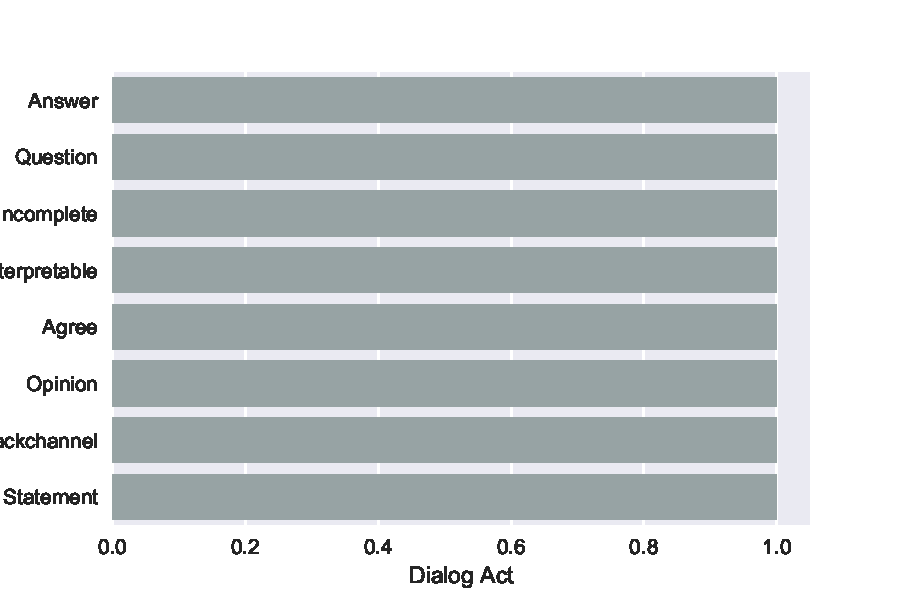
\includegraphics[width=0.5\textwidth]{../scikitlearn/figures/countplot_da_name_count.pdf}
 \caption{Dialog act size\label{overflow}}
 \label{dactsizefig}
 \end{figure}

Figure \ref{dactssecsbyname} shows an histogram of the length in seconds for each dialog act. It is evident that the distribution is left tilted.

 \begin{figure}[ht!]
 \centering
 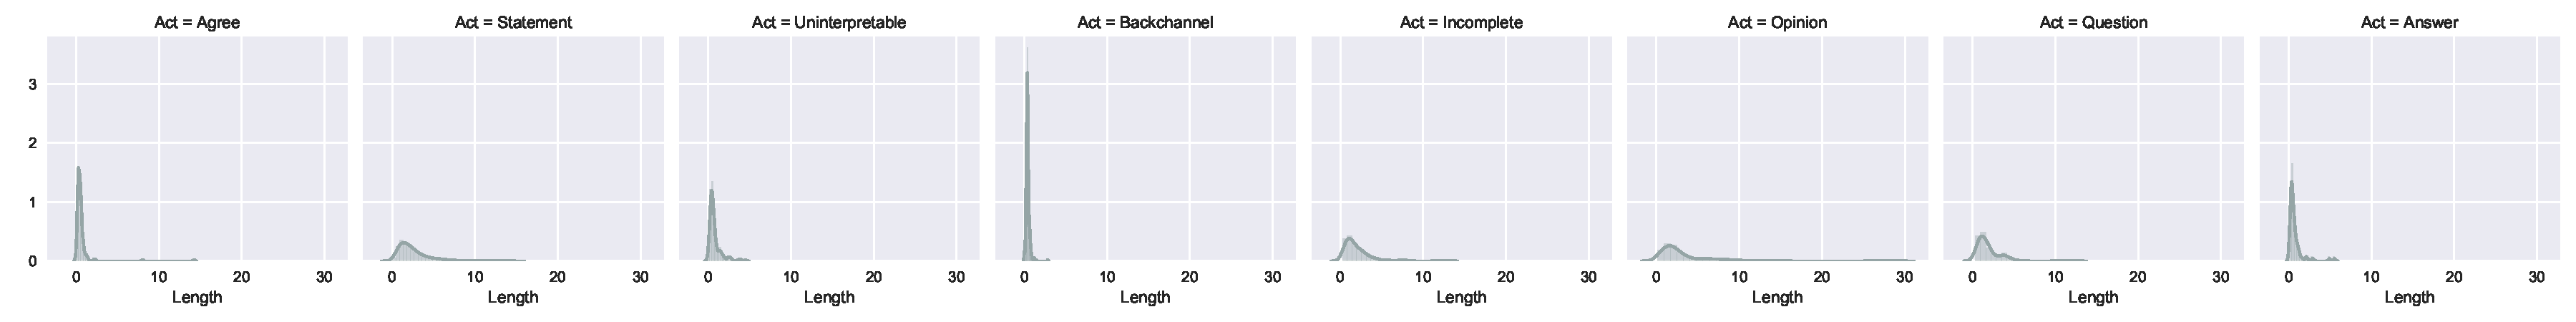
\includegraphics[width=\textwidth]{../scikitlearn/figures/grid_secs_by_da_name.pdf}
 \caption{Dialog act length in words \label{overflow}}
 \label{dactssecsbyname}
  \end{figure}
 
 Figure \ref{l3} shows the and histogram for each dialog act length conditioned on the occuruce of a turn change. We can observe that the length distribution is the same, however when a turn change occur, some
 dialog acts tends to be longer than regular. 
 
\begin{figure}[ht!]
 \centering
 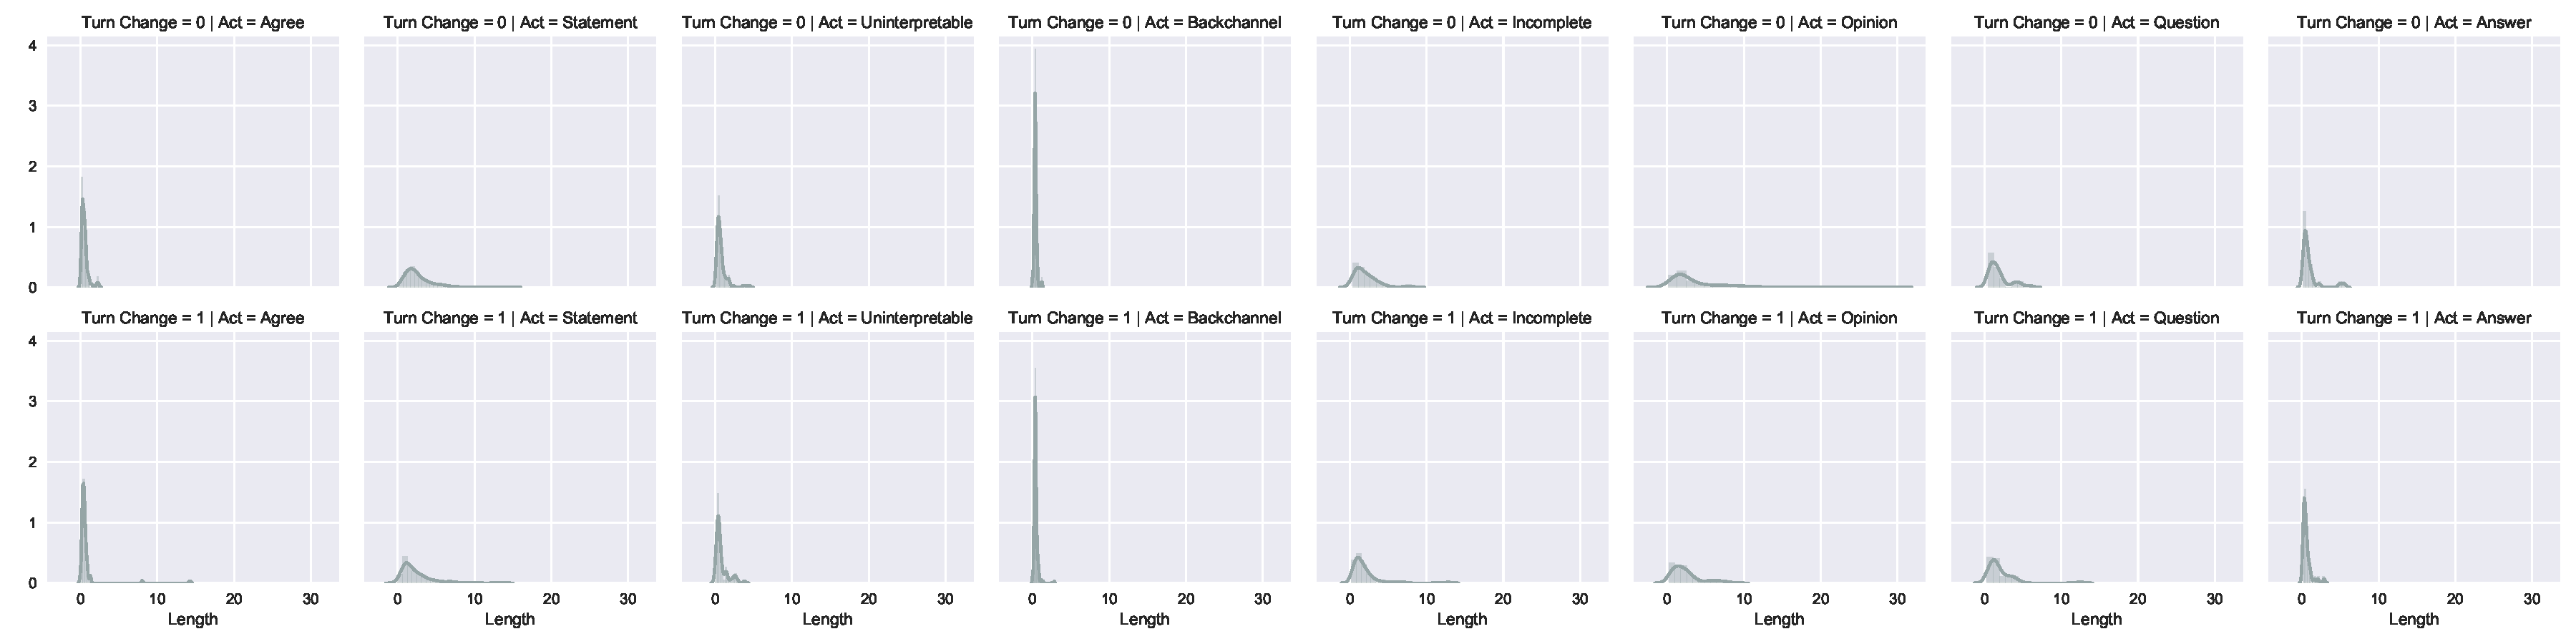
\includegraphics[width=\textwidth]{../scikitlearn/figures/grid_secs_by_da_name_by_tchange.pdf}
 \caption{Dialog act length in words conditioned on turn change\label{overflow}}
 \label{l3}
 \end{figure}
 
In figure \ref{l4} , we measure the probability that a dialog act will lead to turn change. We can observe that the majority of back channels and question will lead to a turn change.  

\begin{figure}[ht!]
\centering
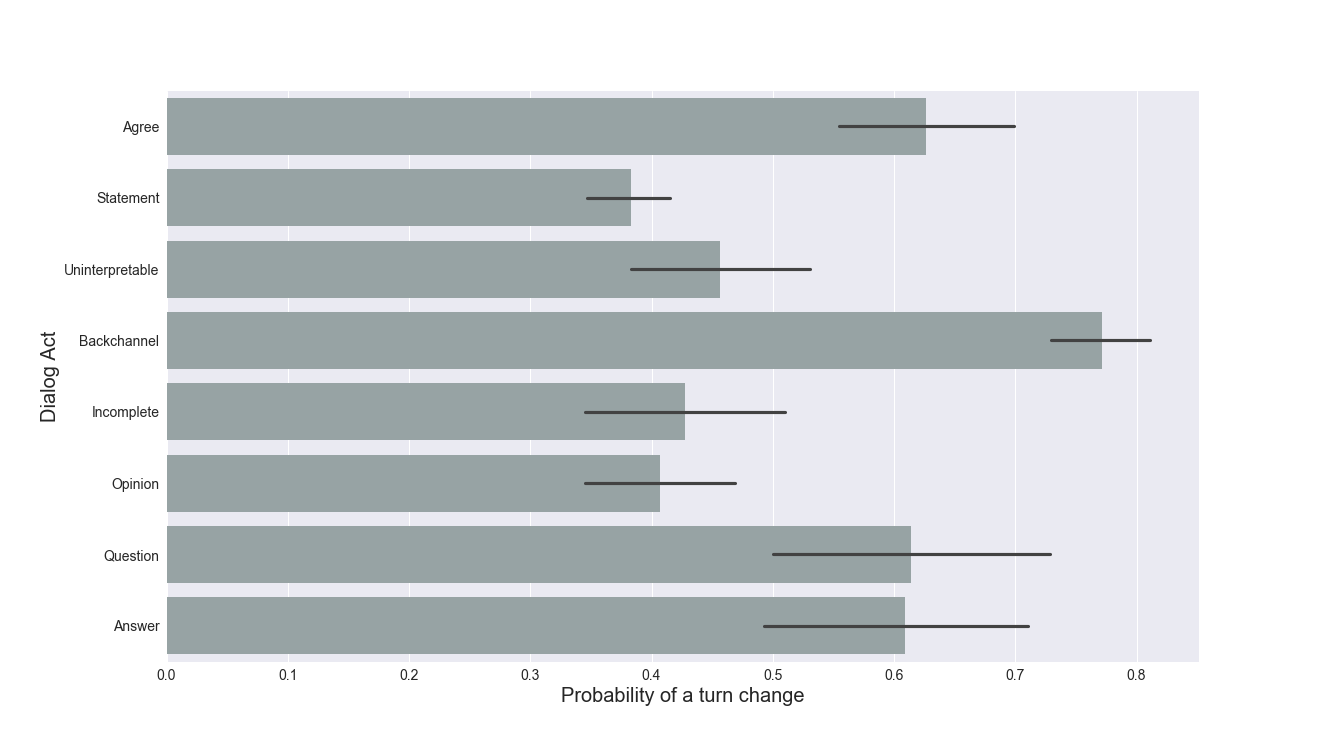
\includegraphics[width=0.5\textwidth]{../scikitlearn/figures/barplot_da_prob_to_tchange.png}
\caption{Dialog act probability of turn change\label{overflow}}
\label{l4}
\end{figure}


\subsection{Relative Turn Length}

Figure \ref{l5} shows the distribution of the relative turn length for each dialog act. We can observe
that 

\begin{figure}[ht!]
\centering
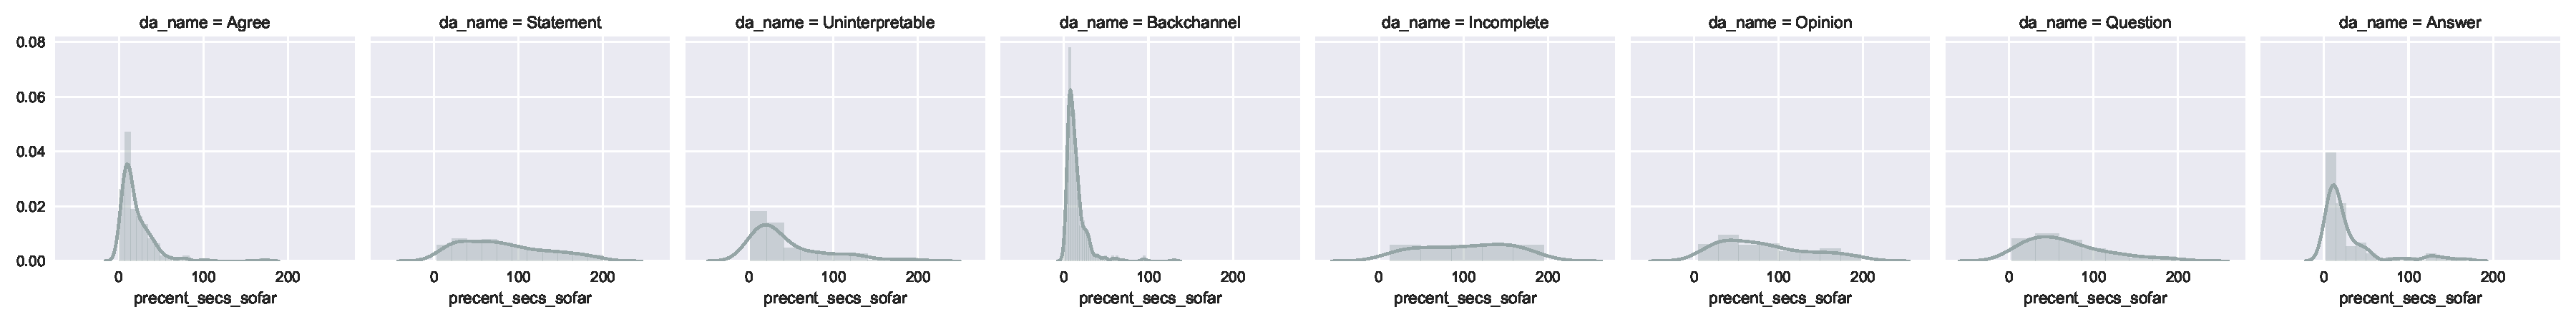
\includegraphics[width=\textwidth]{../scikitlearn/figures/grid_precent_secs_sofar_by_da_name.pdf}
\caption{Relative turn length for each dialog act\label{overflow}}
\label{l5}
\end{figure}
 

\subsection{Relative Floor Control}

Figure \ref{l6} shows distribution of floor control or each dialog act conditioned on a turn change. We can observe that regardless of the dialog act, most distributions are normal with mean of 50\%

\begin{figure}[ht!]
\centering
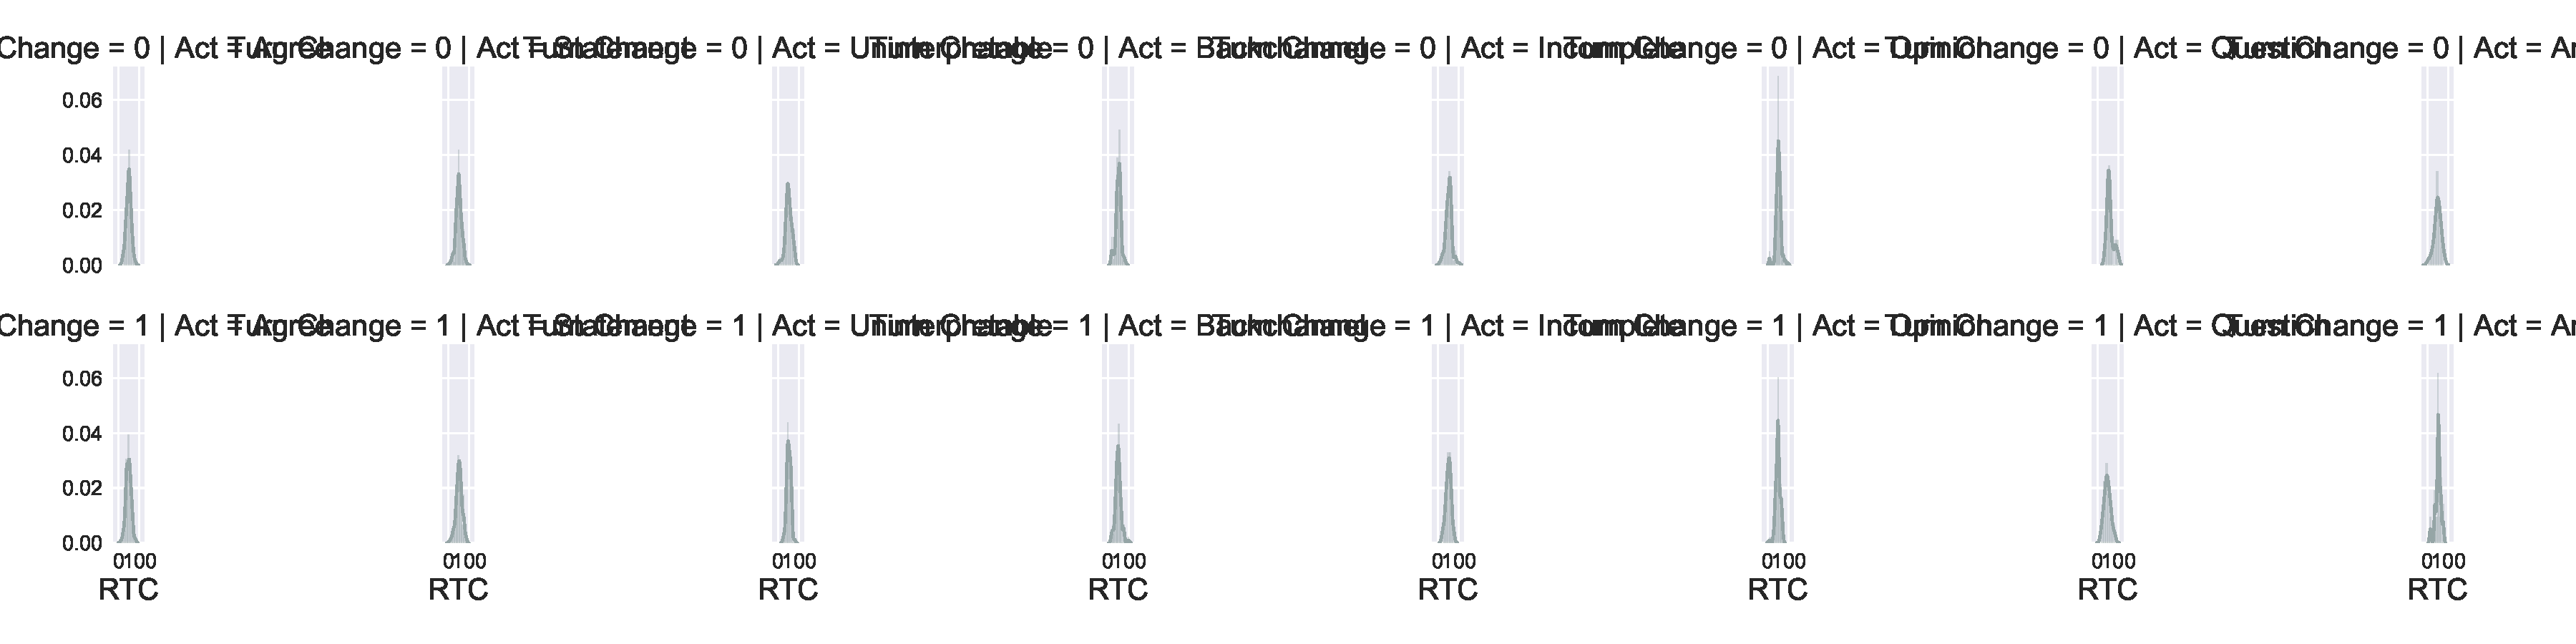
\includegraphics[width=\textwidth]{../scikitlearn/figures/grid_timecontrol_by_da_name_by_tchange.pdf}
\caption{Relative flow control conditioned on turn change\label{overflow}}
\label{l6}
\end{figure}



\subsection{Explanation of the correlation between Relative turn length and turn changes}
\label{sec:opposite}

Our initial hypothesis \ref{chap:intorduction} was that low relative turn change would lead to a speaker holding the floor, and high relative turn change would lead to a turn change. However, in section \ref {sec:data:summary}, we reported that the relative turn length feature was giving us the opposite effect.
We found that the chance of turn change is higher when the speaker has the floor for shorter than its average turn. Also, the speaker will likely keep the floor when speaking more than the average turn length.

We suspect that the reason that our initial hypothesis proved to be incorrect is due to the nature of the corpus. Figure \ref {fig:turn_dist} shows the actual distribution of turn lengths (in seconds).

\begin{figure}[ht!]
\centering
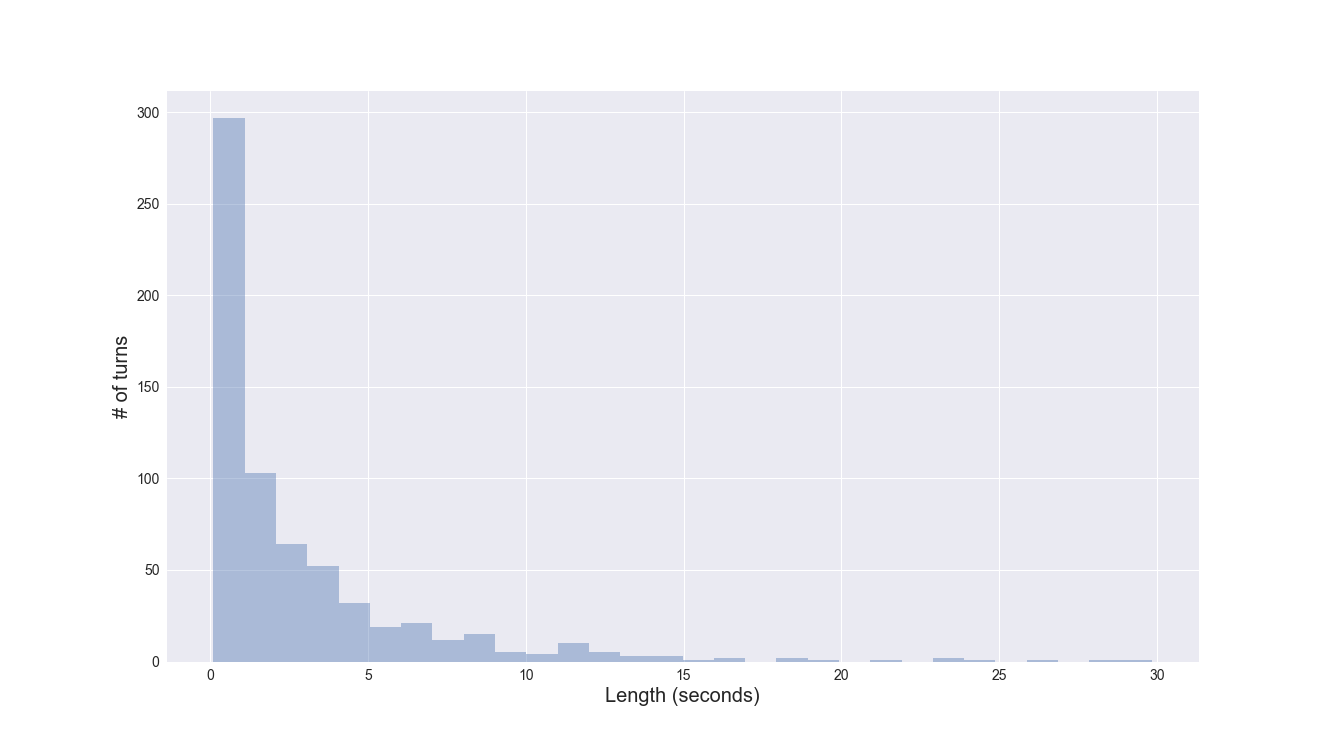
\includegraphics[width=\textwidth]{../scikitlearn/figures/f10.png}\vspace{-1em}
\caption{Distribution of the turn length}
\label{fig:turn_dist}
\end{figure}
%

First we explain why dialog acts with small relative turn length will more likely lead to a turn change. We suspect that the set of short turns is composed of turns with a single dialog act. Moreover, this dialog act is likely to be back channel or an answer, both of which have low relative turn length, see figure \ref{fig:act:turn:rtl}. If we look at figure \ref{fig:act:turnchange}, we can see that the chance of a back channel or a answer causing a turn change is 60-80\%. From both observation we can conclude that a short dialog act with low relative turn length will likely to lead to a turn change.

On the other end, we want to explain why high relative turn length would not lead to a turn change. This can be attributed to the structure of the distribution curve of figure \ref{fig:turn_dist}, which has a long flat tail. Hence if the speaker spoke for high relative turn length, the chance that the current dialog act will lead to a turn change are smaller and smaller and hence the speaker will likely keep the floor.

\chapter {Study}
\subsection{Classification Models}

    To test the contribution of the summary features, we used a binary classifier with
    $y_i$ as the outcome variable. We trained four models, which used the following sets of features:

    \begin{description}
        \item[baseline 1:] Predict turn transition based only on the current dialog act label.
        \item[baseline 2:] Predict turn transition based on the labels of the current and previous dialog acts.
        \item[summary model:] Predict turn transition using just the summary features.
        \item[full model:] Predict turn transition using the summary features and the current and previous dialog acts.
    \end{description}


We used random forests to build the binary classifiers $(N=200)$ \cite{Breiman01randomforests}. Random forests build an ensemble of decision trees during training, and during testing, each decision tree votes on the outcome.  Like decision trees, they can account for interactions between variables, such as making greater use of the summary features when the current speech act is not a question.  Random forests though are not as sensitive to overfitting and data fragmentation.

To find the optimal hyper parameters, we ran a grid search over the \textit{max\_features} and \textit{max\_depth} hyper parameters for each model. The hyper parameters search was done over $\{sqrt, log2, 10\}$ for \textit{max\_features} and $\{5, 7, 9\}$ for \textit{max\_depth}. When training the model, we used the optimal hyper parameters for each feature set.

We performed 10 fold-labeled cross validations.  We made sure that each conversation was entirely in a single fold. This way, each dialogue was entirely used for training or testing, but never for both at the same time.
   
\subsection{Metrics}
After training the models, we perform the actual prediction and evaluate the prediction against the true labels. We than compute the confusion matrix which compose of the following variables.



   
   

\section{Results}
We first analyzed the results in terms of accuracy: how often the models correctly predicted whether a turn transition occurred; in other words, how often the model predicts the correct value of $y_{i+1}$.
%
Table \ref{table:result} shows the results of training a random forest of 200 trees for each model using 10 folds cross validation. We see that using the summary features provides better accuracy than baseline 1, which use only the current dialog act ($65.54\%$ vs $62.79\%$). In addition, using the full model yields an improvement of over $1.08\%$ in the accuracy. In addition, baseline 1 has high precision, it has very low recall. Using only the summary model improves recall and decreases precision by less, leading to a higher F1 score and overall better performance. Using the full model improves precision, which means that dialog acts that were considered to lead to turn transitions are classified correctly. If we use the full model, we lose precision (over baseline 2 model), but gain recall,
leading to the highest F1 score and the best performance.
%
\begin{table}[ht!]
\begin{center}
\begin{tabular}{lrrrrr}
\toprule
{} &  Accuracy &        F1 &  Precision &    Recall &   AUC \\
\midrule
baseline 1 &  0.627938 &  0.578149 &   0.749824 &  0.470491 &  0.659992 \\
baseline 2 &  0.748900 &  0.748792 &   0.818479 &  0.690012 &  0.811185 \\
summary    &  0.655471 &  0.693203 &   0.672255 &  0.713612 &  0.694657 \\
full       &  0.757515 &  0.775993 &   0.775099 &  0.778319 &  0.837863 \\
\bottomrule
\end{tabular}
\end{center}
\caption{Precision, recall and F1 results using Random Forests }
\label{table:result}
\end{table}


The effect can also be seen in figure \ref{auc}, which shows the ROC curves and the AUC for each
model. We notice that the AUC of the summary model is better than baseline 1 model ($0.69$ vs $0.66$), and when adding the summary features to the local features (the full model), we see the AUC improves ($0.84$ vs $0.81$). This suggests that while the discrimination facility of the summary features is lacking (AUC $<0.7$), adding them to a classifier that uses local features (full model) yields better results than the baseline.
%
 \begin{figure}[ht!]
 \centering
 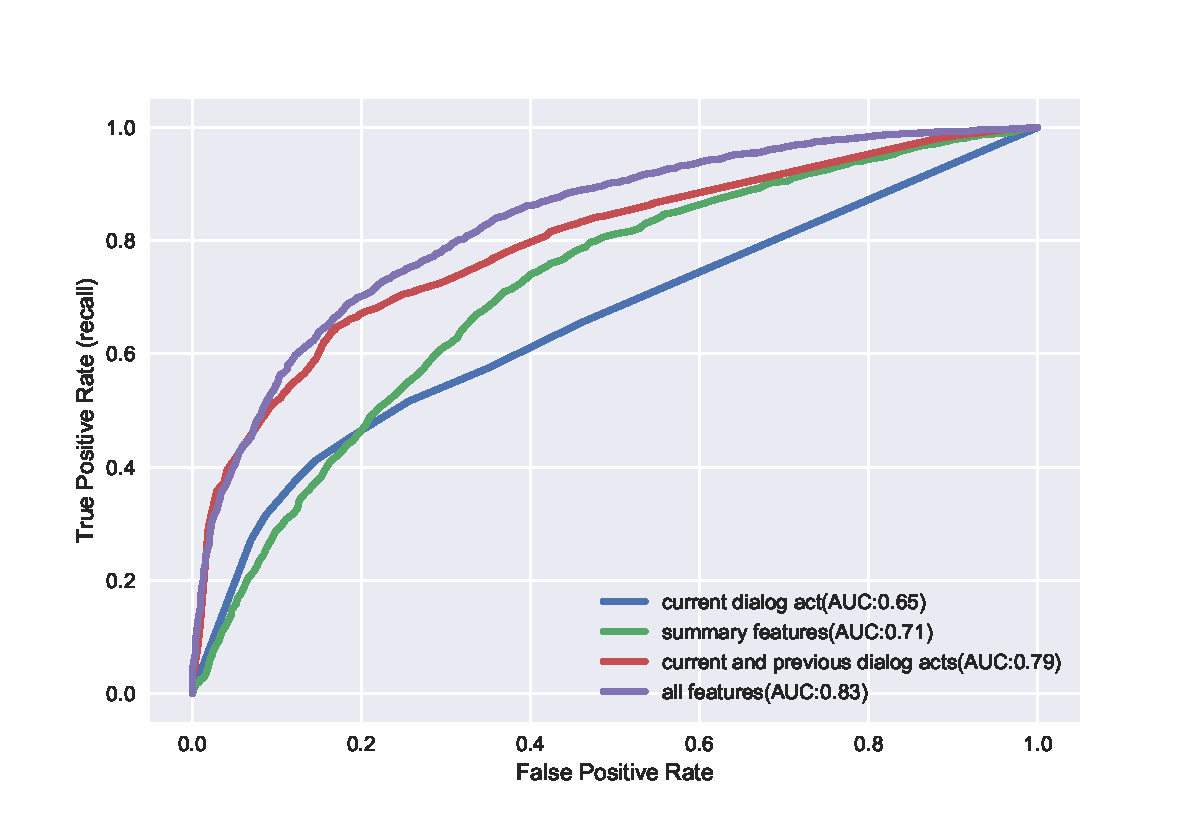
\includegraphics[width=\textwidth]{../scikitlearn/figures/roc.pdf}\vspace{-1.5em}
 \caption{ROC curves and AUC of the different models \label{overflow}}
\label{auc}
 \end{figure}


\begin{table}[ht!]
\begin{center}
\begin{tabular}{lrrrrr}
\toprule
{} &  accuracy &        f1 &  precision &    recall &   roc\_auc \\
\midrule
all        &  0.765718 &  0.787481 &   0.774492 &  0.801152 &  0.848495 \\
baseline 1 &  0.627938 &  0.578149 &   0.749824 &  0.470491 &  0.659992 \\
baseline 2 &  0.748834 &  0.748210 &   0.819280 &  0.688687 &  0.811097 \\
summary    &  0.679110 &  0.713018 &   0.692053 &  0.735588 &  0.726475 \\
\bottomrule
\end{tabular}
\end{center}
\caption{Precision, recall and F1 results using Random Forests }
\label{table:result}
\end{table}


\subsection{Sensitivity to measurement start time}

In Meshorer and Heeman \cite{Meshorer2016UsingPS} we assumed that it take 120 seconds for the conversational image to form. To validate this assumption here, we computed the AUC for the different model using different starting time. Table \ref{table:starttime} shows that the AUC values stay consistent with using different start times. This shows that the summary features predictive strengh is not affected by the start time.

%
\begin{table}[ht!]
\begin{center}
\begin{tabular}{lrrrrrrr}
\toprule
{} & 0 & 15 & 30 & 45 & 60 & 120 & 180  \\
\midrule
baseline 1 & 0.659992 & 0.661070 & 0.661265 & 0.660901  & 0.660261 & 0.659855 & 0.660598  \\
baseline 2 & 0.811185 & 0.812167 & 0.812493 & 0.812012  & 0.811513 & 0.809206 & 0.806845  \\
summary    & 0.694657 & 0.695172 & 0.694351 & 0.694907  & 0.695737 & 0.691010 & 0.692128  \\
all        & 0.837863 & 0.838777 & 0.838533 & 0.838016  & 0.836148 & 0.831940 & 0.828085  \\

\bottomrule
\end{tabular}
\end{center}
\caption{ AUC Score in relation to the start of the dialog }
\label{table:starttime}
\end{table}




\chapter{Conclusions}
This paper explores the use of features that capture speakers' past turn-taking behavior in predicting whether their will be a turn transition.  These summary features include (a) relative turn length: how the current turn under construction compares to the current speaker's average turn length; and (b) relative floor control: the percentage of time that the current speaker has held the floor.  We include two versions of each, one based on time, and one based on number of words.
%
Relative turn length should capture whether one or both of the speakers tends to hold the turn over multiple utterances, while relative floor control captures whether one speaker is dominating the conversation.  Both of these factors should influence who will speak next.

In evaluating our model on data from the Switchboard corpus, we find that our summary features on their own do better than just using the previous speech act (accuracy of $66.14\%$ vs $60.26\%$).  We also find that when we add these features to a model that uses the last two speech acts, we also see an improvement ($76.05\%$ vs $74.43\%$).  These results show the potential of modeling speakers' past turn-taking behavior in predicting upcoming turn-transitions.  Better modeling of turn-taking should lead to more natural and efficient spoken dialogue systems.

\section{Future Direction}
In this work, the local features that we considered in our baseline model were just the last two speech acts.  Other work on turn-taking prediction use a richer set of local features, such as
%
syntactic \cite{ duncan1972some, sacks1974simplest, ford1996interactional, de2006projecting, magyari2012prediction, atterer2008towards}, prosodic \cite{ duncan1972some, ford1996interactional, shriberg2000prosody, ferrer2003prosody, de2006projecting, reed2009units, raux2012optimizing, hariharan2001robust, atterer2008towards}, pragmatic \cite{ ford1996interactional, garrod2015use, raux2012optimizing}, semantic \cite{raux2012optimizing} and non verbal \cite{kendon1967some}. In future work, it would be good to evaluate the contribution of our summary features with a richer set of local features.

In our work, we evaluated our model on the Switchboard corpus.  In future work, it would also be good to evaluate our summary features on other corpora, especially task-based dialogues.  Tasks in which there is a difference in the role of the user and speaker, such as in Trains \cite{HeemanAllen95:cdrom}, should benefit from modeling the past turn-taking behavior of each speaker.

More generally, the summary features introduced in this work represent just one aspect of the conversational image of the user. Future work should try to ``summarize'' other local features by creating
the average value of a local feature over past turns. For example, we can compute relative speech rate, or relative use of stereotyped expressions.



% Appendix
\appendix


% Bibliography
\nocite{*} % temporarily include all references, even if not cited
\bibliographystyle{abbrv} % check with your advisor for appropriate style
\bibliography{thesis} % name of your thesis.bib file


% Biographical note
%\biography
%\lipsum[9]


\end{document}
